\documentclass[a4paper,11pt,openany]{ltjsreport}

% ============================================================
% フォント設定
% ============================================================
\usepackage{luatexja-fontspec}

\setmainfont{TeX Gyre Termes}
\setsansfont{TeX Gyre Heros}
\setmainjfont[
  BoldFont=Harano Aji Mincho Bold,
  ItalicFont=Harano Aji Mincho,
  BoldItalicFont=Harano Aji Mincho Bold
]{Harano Aji Mincho}

% ============================================================
% レイアウト
% ============================================================
\usepackage[top=25mm,bottom=25mm,left=25mm,right=25mm,bindingoffset=0mm]{geometry}
\usepackage{indentfirst}

% ============================================================
% 汎用パッケージ
% ============================================================
\usepackage{pdfpages}
\usepackage{siunitx}
\usepackage{enumitem}
\usepackage{graphicx}
\usepackage{amsmath}
\usepackage[normalem]{ulem}
\usepackage{url}
\usepackage{float}
\usepackage{amssymb}

% ============================================================
% 句読点変換設定 (Lua)
% ============================================================
\usepackage{luatexja}
\directlua{
  local function replace_punctuation(s)
    s = s:gsub("、", "，")
    s = s:gsub("。", "．")
    return s
  end
  luatexbase.add_to_callback("process_input_buffer", replace_punctuation, "replace_punctuation")
}

% ============================================================
% 表組み・図
% ============================================================
\usepackage{makecell}
\usepackage{hhline}
\usepackage{tabularray}
\usepackage{diagbox}
\usepackage{tikz}
\usepackage[framemethod=TikZ]{mdframed}
\makeatletter
\def\caption@documentclass{standard}
\makeatother
\usepackage{caption}
\usepackage{pifont}
\usepackage{varwidth}

% ============================================================
% 見出しスタイル・カラー・コードリスト
% ============================================================
\usepackage{titlesec}
\usepackage[dvipsnames]{xcolor}
\usepackage{listings}

% ============================================================
% 参考文献
% ============================================================
\usepackage[
  backend=biber,
  style=numeric,
  sorting=none,
  date=iso,
  urldate=iso,
  seconds=true,
  bibencoding=utf8
]{biblatex}
\addbibresource{ref/references.bib}

\DeclareFieldFormat*{title}{#1}
\DeclareFieldFormat*{journaltitle}{#1}
\DeclareFieldFormat*{booktitle}{#1}
\DeclareFieldFormat{url}{\url{#1}}
\DeclareDelimFormat{multinamedelim}{，}
\DeclareDelimFormat{finalnamedelim}{，}
\DefineBibliographyStrings{english}{
  urlseen = {参照},
}
\DeclareFieldFormat[article,inproceedings,misc]{title}{"#1"}
\DeclareFieldFormat[book,inbook]{title}{"#1"}

\DeclareFieldFormat{edition}{#1\addthinspace ed.}

% ============================================================
% キャプション日本語化
% ============================================================
\captionsetup[figure]{name=図}
\captionsetup[table]{name=表}
\captionsetup{labelsep=colon}

% ============================================================
% 図表・数式番号形式
% ----
% \chapter なし（図1 形式）→ 下記ブロックをそのまま使用
% \chapter あり（図1.1 形式）→ 下記ブロックを丸ごとコメントアウト
% ============================================================
\makeatletter
\@removefromreset{section}{chapter}
\@removefromreset{figure}{chapter}
\@removefromreset{table}{chapter}
\@removefromreset{equation}{chapter}
\makeatother
\renewcommand{\thesection}{\arabic{section}}
\renewcommand{\thefigure}{\arabic{figure}}
\renewcommand{\thetable}{\arabic{table}}
\renewcommand{\theequation}{\arabic{equation}}
% ============================================================

% ============================================================
% 見出しフォントサイズ・スペーシング
% ============================================================
\titleformat{\chapter}[block]
  {\fontsize{16pt}{18pt}\selectfont\bfseries}
  {第\thechapter 章\quad}
  {0pt}{}
\titlespacing*{\chapter}{0pt}{20pt}{15pt}

\titleformat{\section}
  {\normalsize\selectfont\bfseries}
  {(2-\thesection)\quad}
  {0pt}{}
\titlespacing*{\section}{0pt}{15pt}{3pt}

% subsection を、()付き小文字ローマン数字に変更。
\renewcommand{\thesubsection}{(\roman{subsection})}

\titleformat{\subsection}
  {\normalsize\selectfont\bfseries}
  {\thesubsection\quad}
  {0pt}{}
\titlespacing*{\subsection}{0pt}{10pt}{3pt}

\titleformat{\subsubsection}
  {\normalsize\bfseries}
  {\thesubsubsection\quad}
  {0pt}{}

\setcounter{secnumdepth}{3}

% ============================================================
% listings カラー定義
% ============================================================
\definecolor{codebg}{RGB}{245,245,245}
\definecolor{identifiercolor}{RGB}{7,54,66}
\definecolor{commentcolor}{RGB}{88,110,117}
\definecolor{framecolor}{RGB}{200,200,200}
\definecolor{keywordcolor}{RGB}{38,139,210}
\definecolor{builtincolor}{RGB}{133,153,0}
\definecolor{stringcolor}{RGB}{42,161,152}

% ============================================================
% listings スタイル定義
% ============================================================
\lstdefinestyle{codestyle}{
  backgroundcolor=\color{codebg},
  basicstyle=\linespread{1.1}\small\ttfamily\color{identifiercolor},
  frame=single,
  framerule=0.5pt,
  rulecolor=\color{framecolor},
  breaklines=true,
  showstringspaces=false,
  numbers=left,
  xleftmargin=2em,
  keywordstyle=\color{keywordcolor}\bfseries,
  stringstyle=\color{stringcolor},
  commentstyle=\color{commentcolor}\itshape,
  numberstyle=\normalsize\color{black},
}

\lstdefinestyle{python}{
  style=codestyle,
  language=Python,
  morekeywords=[2]{self,True,False,None,print,range,len,dict,list,set,zip,
    int,str,float,max,min,open,round,tuple,Exception,ValueError,
    FileNotFoundError,__name__},
  keywordstyle=[2]\color{builtincolor},
}

\lstdefinestyle{cpp}{
  style=codestyle,
  language=C++,
  morekeywords=[2]{
    nullptr,bool,true,false,
    uint8_t,uint16_t,uint32_t,
    int8_t,int16_t,int32_t,
    size_t,String,
    setup,loop,
    pinMode,digitalWrite,digitalRead,
    analogRead,analogWrite,
    delay,delayMicroseconds,
    millis,micros,
    HIGH,LOW,INPUT,OUTPUT,INPUT_PULLUP,
    Serial,begin,print,println,write,available,read,
    SoftwareSerial
  },
  keywordstyle=[2]\color{builtincolor},
}

\lstset{style=python}

% コードブロックの日本語化
\renewcommand{\lstlistingname}{コード}
\renewcommand{\lstlistlistingname}{コード一覧}

% ============================================================
% siunitx
% ============================================================
\sisetup{
  detect-all,
  mode=math
}

% ============================================================
% hyperref
% ============================================================
\usepackage{hyperref}
\hypersetup{
  colorlinks=true,
  linkcolor=black,
  urlcolor=black,
  citecolor=black,
  bookmarksnumbered=true,
  pdfborder={0 0 0},
  pdfencoding=auto,
  pdftitle={レポート},
  pdfauthor={中山 将吾}
}

\begin{document}

\setcounter{page}{1}

% ============================================================
% 表紙（どちらか一方を有効化）
% ============================================================

% -- 指定表紙PDFを使う場合（通常はこちら） --
% \includepdf{./cover.pdf}

% -- 自作表紙を使う場合はコメントを外す --
\begin{titlepage}
	\vspace*{\stretch{1.0}}
	\begin{flushright}
		\large{提出日: 2026年5月17日}
	\end{flushright}
	\vspace*{\stretch{2.3}}
	\begin{center}
		{\huge オペレーティングシステム} \\
		{\vspace{1cm}}
		{\huge レポート課題2 (2-1)}
	\end{center}
	\vspace*{\stretch{3.0}}
	\begin{center}
		{\large 所属: 電子情報工学科・4年} \\
		\vspace{0.5cm}
		{\large 学籍番号: i231331} \\
		\vspace{0.5cm}
		{\large 出席番号: 33番} \\
		\vspace{0.5cm}
		{\large 氏名: 中山 将吾}
	\end{center}
	\vspace*{\stretch{1.0}}
\end{titlepage}

\section{以下の処理の時系列遷移を示したうえで、a, b に適切な数字を埋めよ。}
四つのプロセス A \textasciitilde D があり、各プロセスの到着時間と処理時間を表\ref{tab:question}に示す。
表において、到着時刻とは、プロセス A が待ち行列に到着した時刻を0としたときの各プロセスが到着する時間であり、処理時間とは、各プロセスの処理が完了する為に必要な CPU の処理時間である。

このとき、到着順方式におけるターンアラウンドタイムの平均は [a] ミリ秒である。
そして、タイムクウォンタムが20ミリ秒のとき、ラウンドロビン方式におけるターンアラウンドタイムの平均は [b] ミリ秒である。
ここで、プロセス A が到着したとき、実行可能状態及び実行状態のプロセスはないものとする。
なお、プロセスの登録と取出し、及び中断の処理でのオーバヘッドは考えない。
また、CPU を割り当てられたプロセスは、タイムクウォンタム以外で中断することはない。

\begin{table}[H]
	\centering
	\caption{各プロセスの到着時刻と処理時間}
	\label{tab:question}
	\begin{tabular}{|c|c|c|}
		\hline
		プロセス & 到着時刻 (ミリ秒) & 処理時間 (ミリ秒) \\
		\hline
		A    & 0          & 80         \\
		\hline
		B    & 20         & 60         \\
		\hline
		C    & 40         & 70         \\
		\hline
		D    & 70         & 50         \\
		\hline
	\end{tabular}
\end{table}

% 解答
\subsection{到着順方式}
到着順方式におけるプロセスの時系列遷移を図\ref{fig:fcfs}に示す。

\begin{figure}[H]
	\centering
	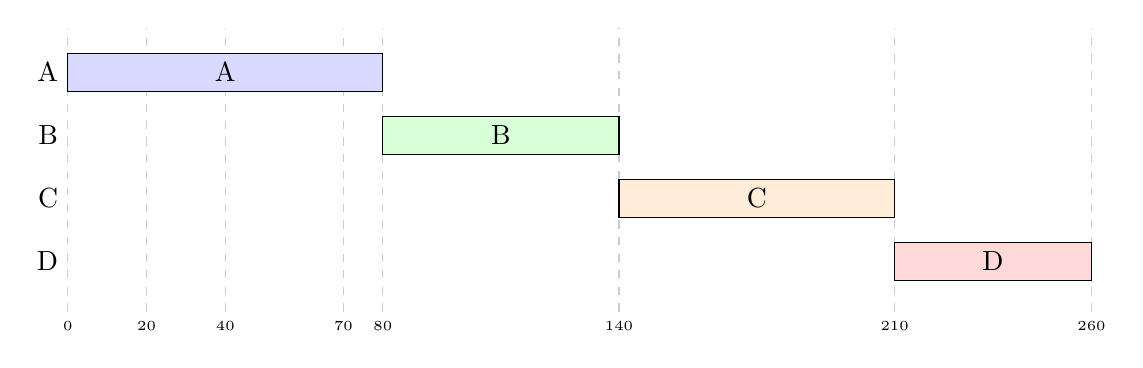
\begin{tikzpicture}[x=0.05cm, y=0.8cm]
		\foreach \x in {0, 20, 40, 70, 80, 140, 210, 260} {
				\draw[dashed, gray!40] (\x, -0.5) -- (\x, 4);
				\node[below, font=\tiny] at (\x, -0.5) {\x};
			}
		\draw[fill=blue!15] (0,3) rectangle (80,3.6) node[pos=.5] {A};
		\node[left] at (0,3.3) {A};
		\draw[fill=green!15] (80,2) rectangle (140,2.6) node[pos=.5] {B};
		\node[left] at (0,2.3) {B};
		\draw[fill=orange!15] (140,1) rectangle (210,1.6) node[pos=.5] {C};
		\node[left] at (0,1.3) {C};
		\draw[fill=red!15] (210,0) rectangle (260,0.6) node[pos=.5] {D};
		\node[left] at (0,0.3) {D};
	\end{tikzpicture}
	\caption{到着順方式におけるプロセスの時系列遷移}
	\label{fig:fcfs}
\end{figure}

図\ref{fig:fcfs}より、各プロセスのターンアラウンドタイムは、

\begin{itemize}
	\item プロセス A: $80 - 0 = 80$ ミリ秒
	\item プロセス B: $140 - 20 = 120$ ミリ秒
	\item プロセス C: $210 - 40 = 170$ ミリ秒
	\item プロセス D: $260 - 70 = 190$ ミリ秒
\end{itemize}

である。
よって、平均ターンアラウンドタイムは、

\begin{align*}
	\frac{80 + 120 + 170 + 190}{4} = 140
\end{align*}

より、$\text{[a]} = 140$ ミリ秒である。

\clearpage

\subsection{ラウンドロビン方式}
ラウンドロビン方式におけるプロセスの時系列遷移を図\ref{fig:rr}に示す。

\begin{figure}[H]
	\centering
	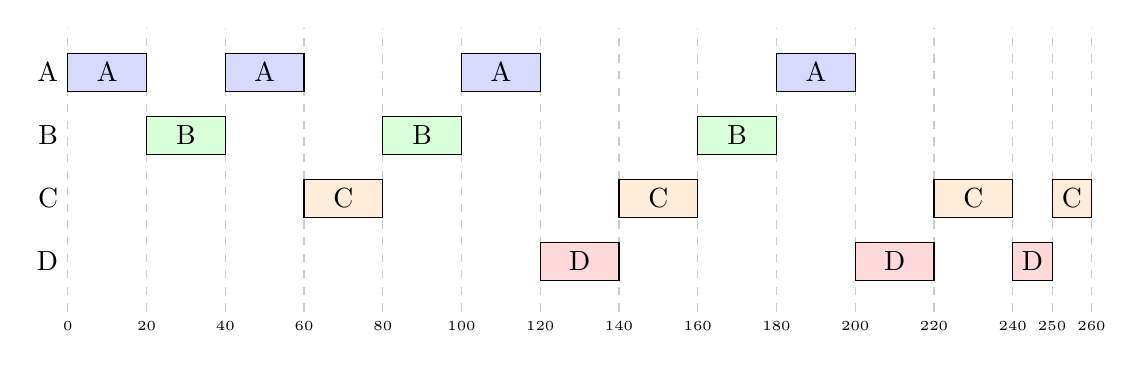
\begin{tikzpicture}[x=0.05cm, y=0.8cm]
		\foreach \x in {0, 20, 40, 60, 80, 100, 120, 140, 160, 180, 200, 220, 240, 250, 260} {
				\draw[dashed, gray!40] (\x, -0.5) -- (\x, 4);
				\node[below, font=\tiny] at (\x, -0.5) {\x};
			}
		\draw[fill=blue!15] (0,3) rectangle (20,3.6) node[pos=.5] {A};
		\draw[fill=blue!15] (40,3) rectangle (60,3.6) node[pos=.5] {A};
		\draw[fill=blue!15] (100,3) rectangle (120,3.6) node[pos=.5] {A};
		\draw[fill=blue!15] (180,3) rectangle (200,3.6) node[pos=.5] {A};
		\node[left] at (0,3.3) {A};

		\draw[fill=green!15] (20,2) rectangle (40,2.6) node[pos=.5] {B};
		\draw[fill=green!15] (80,2) rectangle (100,2.6) node[pos=.5] {B};
		\draw[fill=green!15] (160,2) rectangle (180,2.6) node[pos=.5] {B};
		\node[left] at (0,2.3) {B};

		\draw[fill=orange!15] (60,1) rectangle (80,1.6) node[pos=.5] {C};
		\draw[fill=orange!15] (140,1) rectangle (160,1.6) node[pos=.5] {C};
		\draw[fill=orange!15] (220,1) rectangle (240,1.6) node[pos=.5] {C};
		\draw[fill=orange!15] (250,1) rectangle (260,1.6) node[pos=.5] {C};
		\node[left] at (0,1.3) {C};

		\draw[fill=red!15] (120,0) rectangle (140,0.6) node[pos=.5] {D};
		\draw[fill=red!15] (200,0) rectangle (220,0.6) node[pos=.5] {D};
		\draw[fill=red!15] (240,0) rectangle (250,0.6) node[pos=.5] {D};
		\node[left] at (0,0.3) {D};
	\end{tikzpicture}
	\caption{ラウンドロビン方式におけるプロセスの時系列遷移}
	\label{fig:rr}
\end{figure}

図\ref{fig:rr}より、各プロセスのターンアラウンドタイムは、

\begin{itemize}
	\item プロセス A: $200 - 0 = 200$ ミリ秒
	\item プロセス B: $180 - 20 = 160$ ミリ秒
	\item プロセス C: $260 - 40 = 220$ ミリ秒
	\item プロセス D: $250 - 70 = 180$ ミリ秒
\end{itemize}

である。よって、平均ターンアラウンドタイムは、

\begin{align*}
	\frac{200 + 160 + 220 + 180}{4} = 190
\end{align*}

より、$\text{[b]} = 190$ ミリ秒である。

% \printbibliography[title=参考文献]

\end{document}
